
% \documentclass[blackref,approvalform,dvipsnames]{drexel-thesis}
\documentclass[draft,dvipsnames]{drexel-thesis}


\author{Jae Hoon Kim}
\title{Classifying Human Driving Behavior via Deep Neural Networks}
\DUTmonth{June}
\DUTyear{2017}
\degree{Master in Computer Science}
\advisor{Santiago~Onta\~{n}\'{o}n, Ph.D.}
\copyrighttext{\copyrighttextCCBYSA}

\usepackage[numbers,sort&compress]{natbib} % fancy citation extensions
\bibliographystyle{unsrtnat}


% \usepackage{fancyvrb} % nicer verbatim handling
% \DefineShortVerb{\|}  % \verb+TEXT+  ->  |TEXT|

\usepackage{xcolor}
\usepackage{colortbl,booktabs}
\usepackage{xspace}
\usepackage{multirow}
\usepackage{wrapfig} % text around figures
\usepackage{amssymb} % \mathbbstarcra
\usepackage[final]{listings} % algorithms formated in code
\usepackage{enumitem} % compact imte lists
\usepackage{subcaption} % for subfigure (figures side-by-side)
\usepackage{mathtools}
\usepackage{soul}
\usepackage[detect-all]{siunitx} % Aligning numbers by decimal points in table columns
\usepackage{bm}

\usepackage{algorithm, soul}
\usepackage[noend]{algpseudocode}
\algnewcommand{\Break}{\textbf{break}}

\newcommand{\todo}[1]{{\color{red}{\tt #1}}}
% \newcommand{\toredo}[1]{{\leavevmode\color{Plum}#1}}
\newcommand{\toredo}[1]{#1}
\newcommand{\modified}[1]{{\leavevmode\color{blue}#1}}
% \newcommand{\modified}[1]{#1}
\newcommand{\highest}[1]{\textcolor{Maroon}{\textbf{#1}}}
\newcommand{\StarCraft}{\mbox{\textsc{StarCraft}}\xspace}
\newcommand{\BroodWar}{\textsc{StarCraft: Brood War}\xspace}
\newcommand{\WarCraft}{\mbox{\textsc{WarCraft}}\xspace}
\newcommand{\WarCraftII}{\mbox{\textsc{WarCraft II}}\xspace}
\newcommand{\WarCraftIII}{\mbox{\textsc{WarCraft III}}\xspace}
\newcommand{\Wargus}{\mbox{\textsc{Wargus}}\xspace}
\newcommand{\Spring}{\mbox{\textsc{Spring}}\xspace}
\newcommand{\BWTA}{\textsc{BWTA}\xspace}
\newcommand{\BWTAb}{\textsc{BWTA2}\xspace}
\newcommand{\BWAPI}{\textsc{BWAPI}\xspace}
\newcommand{\SparCraft}{\textsc{SparCraft}\xspace}
\newcommand{\Lanchester}{\mbox{\emph{TS-Lanchester}$^2$}\xspace}
\newcommand{\cop}{\textsc{COP}\xspace}
\newcommand{\Ghost}{\textsc{GHOST}\xspace}
\newcommand{\Nova}{\textsc{Nova}\xspace}




\begin{document}
\begin{preamble}

% \begin{dedications}
% We're in \iffinal{final}{draft} mode!
% \end{dedications}

% \begin{acknowledgments}
% bla bla bla
% \end{acknowledgments}

\tableofcontents
\listoftables
\listoffigures

% \iffinal{}{\newpage}

\begin{abstract}
The average person spends several hours a day behind the wheel of their vehicles, which are usually equipped with on-board computers capable of collecting real-time data concerning driving behavior. However, this data source has rarely been tapped for healthcare and behavioral research purposes. This MS thesis is done in the context of the {\em Diagnostic Driving} project, an NSF funded collaborative project between Drexel, Children Hospital of Philadelphia (CHOP) and the University of Central Florida that aims at studying the possibility of using driving behavior data to diagnose medical conditions. 
%
Specifically, this paper introduces focuses on the classification of driving behavior data collected in a driving simulator using deep neural networks. The target classification task is to differentiate novice versus expert drivers. The paper presents a comparative study on using different variants of LSTM (Long-Short Term Memory networks) and Auto-encoder networks to deal with the fact that we have a small amount of labels (16 examples of people driving in the simulator, each labeled with an ``expert'' or ``inexpert'' label), but each simulator drive is high dimensional and too densely sampled (each drive consists of 100 variables sampled at 60Hz).
%
Our results show that using an intermediate number of neurons in the LSTM networks and using data filtering (only considering one out of each 10 samples) obtains better results, and that using Auto-encoders works worse than using manual feature selection.
\end{abstract}
\end{preamble}

\begin{thesis}



% ####################################################################################################################################
\chapter{Introduction}\label{chap:intro}
% ####################################################################################################################################

Introduction Section
\begin{enumerate}
\item Problem Statement
\end{enumerate}



% ====================================================================================================================================
% ====================================================================================================================================
\chapter{Background}\label{sec:bg}
% ====================================================================================================================================
% ====================================================================================================================================
This chapter presents the necessary background to understand the experiments presented later in the paper. This chapter is dived into three sections. First Section \ref{sec:DL} covers basic deep learning including recurrent neural network and auto-encoders. Second Section \ref{sec:DLL} compares deep learning libraries: DL4J, Theano, and Tensorflow. The last Section \ref{sec:MLDD} introduces current trends in machine learning for driving data.

\section{Deep Learning}\label{sec:DL}
This section covers basic concepts of deep learning. First Subsection \ref{subsec:basicDL} introduces deep learning, and next Section \ref{subsec:RNN} deals with recurrent neural networks and long short term memory neural networks (LSTMs). The last Subsection \ref{subsec:AE} covers auto-encoders.

\subsection{Basic Concepts}\label{subsec:basicDL}

\subsubsection{Artificial Neuron}\label{subsubsec:AN}
The concept of artificial neurons or perseptrons was introduced by Warren McCullock and Walter Pitts \cite{raschka2015python}. Initial artificial neurons are described as binary output logic gate from inputs. If sum of weighted inputs is greater than threshold, the output is 1. Otherwise, the output is 0.

\begin{figure}[t!]
    \centering
    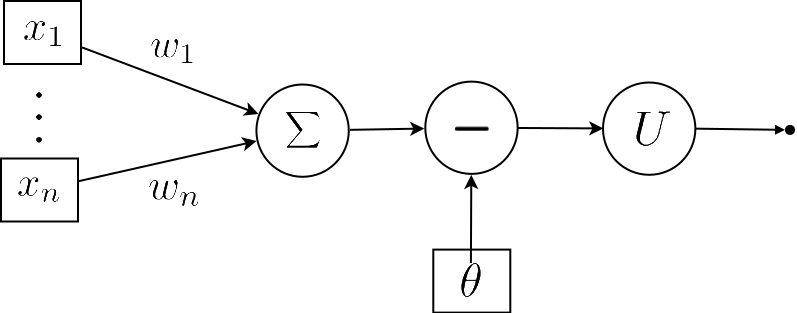
\includegraphics[width=0.65\textwidth]{pictures/figures/basic_AN.png}
    \caption{Basic Artificial Neuron}
    \label{fig:basic_AN}
\end{figure}

Figure \ref{fig:basic_AN} shows a basic artificial neuron. The input is $\vec{x} = \{x_1, ..., x_n\} \in \mathbb{R}^n$ and the weights for each input are $\vec{w} = \{w_1, ..., w_n\} \in \mathbb{R}^n$. Let $\theta$ be threshold and define step function as below:

$$U(z)=
	\begin{cases} 
		\hfill 1 \hfill & \text{if $z > 0$} \\
		\hfill 0 \hfill & \text{otherwise} \\
	\end{cases}
$$

The function deciding output $o$ is called an activation function. In this case, the step function $U(z)$ is activation function.

Figure \ref{fig:basic_AN} also can be described by the following equation:
$$ o = U(\vec{x}\cdot\vec{w}-\theta)$$

\begin{figure}[t!]
    \centering
    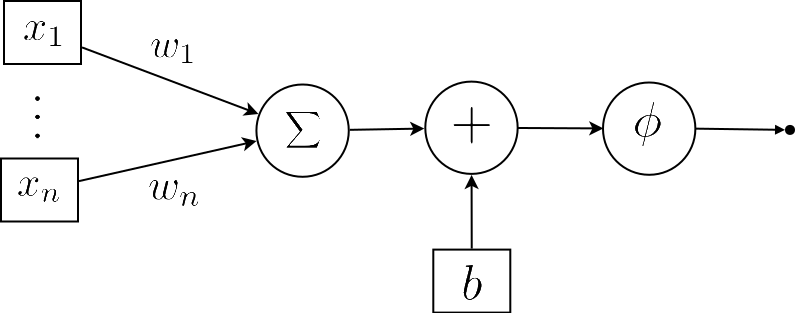
\includegraphics[width=0.65\textwidth]{pictures/figures/general_AN.png}
    \caption{General Artificial Neuron}
    \label{fig:general_AN}
\end{figure}

Figure \ref{fig:general_AN} shows an general artificial neuron. Threshold is replaced by bias and subtract node is replaced by add node. In general artificial neuron, activation function $\phi$ can be many different functions such as step, linear, or sigmoid function. An general artificial neuron also can be described by equation as follow:
$$o = \phi(\vec{x}\cdot\vec{w}+b)$$


\subsubsection{Neural Network}\label{subsubsec:NN}

\begin{figure}[t!]
    \centering
    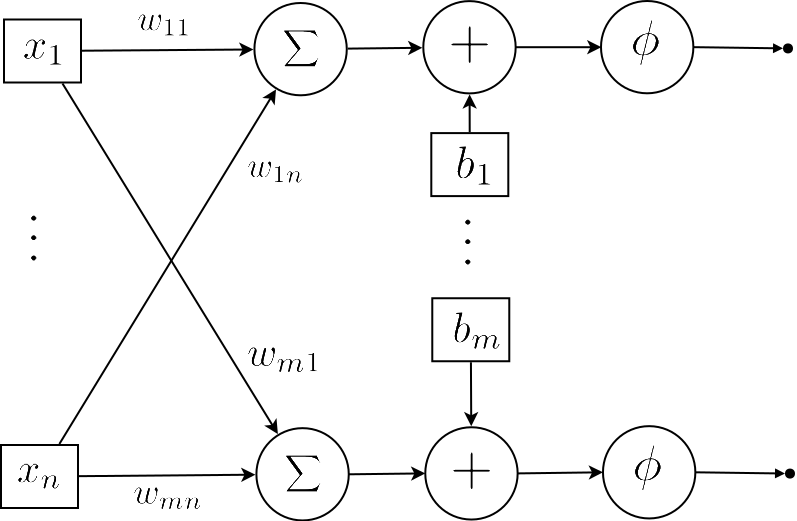
\includegraphics[width=0.65\textwidth]{pictures/figures/detail_NN.png}
    \caption{Single Layer in a Neural Network}
    \label{fig:detail_NN}
\end{figure}

Using single neuron has a limitation since it can solve only specific problems. For example, single neuron cannot solve xor problem. Instead of using single neuron, neural network has bundle of neurons. Figure \ref{fig:detail_NN} illustrates it with $n$ input and $m$ neurons. The input is $\vec{x} = \{x_1, ..., x_n\} \in \mathbb{R}^n$, weights for $i$th neuron are $\vec{w_i} = \{w_{i1}, ..., w_{in}\} \in \mathbb{R}^n$, and a bias term for the $i$th neuron is $b_i$. The output $\vec{o} = \{o_1, ..., o_m\} \in \mathbb{R}^m$ of the network is calculated as follows:
$$\vec{o} = \bm{\phi}(\{(\vec{x}\cdot\vec{w_1}+b_1),(\vec{x}\cdot\vec{w_2}+b_2),...,(\vec{x}\cdot\vec{w_m}+b_m)\})$$
Where activation function is applied on each element of its input.

To simplify the equation, let a transform matrix $\bold{w}: \mathbb{R}^n \rightarrow \mathbb{R}^m$ be
$\bold{w}=
\begin{bmatrix}
	\vec{w_1} & \vec{w_2} & \cdots & \vec{w_m}
\end{bmatrix}$
and bias vector $\vec{b} = \{b_1, ..., b_m\} \in \mathbb{R}^m$.

The equation is
$$\vec{o} = \bm{\phi}((\vec{x}^T\bold{w})^T+\vec{b})$$

The bias term can be skipped by extending input vector and weight transform matrix. Let $\vec{X} \in \mathbb{R}^{n+1}$ be $\{x_1, x_2, ..., x_n, 1\}$ which is added one more dimension from $\vec{x}$ with value 1 and $\vec{W_i} \in \mathbb{R}^{n+1}$ be $\{w_{i1}, ..., w_{in}, b_i\}$ which is added by bias term into weights and $\bold{W}: \mathbb{R}^{n+1} \rightarrow \mathbb{R}^m$ be
$\bold{W}=
\begin{bmatrix}
	\vec{W_1} & \vec{W_2} & \cdots & \vec{W_m}
\end{bmatrix}$

\begin{figure}[t!]
    \centering
    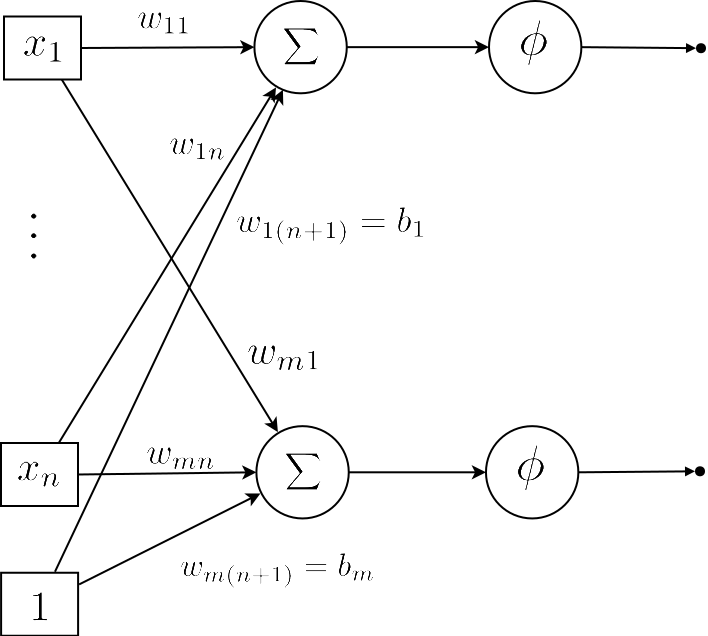
\includegraphics[width=0.75\textwidth]{pictures/figures/detail_NN_with_bias.png}
    \caption{Simplified Neural Network}
    \label{fig:withoutBiasNN}
\end{figure}

Figure \ref{fig:withoutBiasNN} shows same neural network as Figure \ref{fig:detail_NN} with $\vec{X}$ and $\bold{W}$. Notice that the figure does not have an added node anymore.

	From this point on the paper, vector in large case is with bias term and vector in small case is without bias term. For example, $\vec{X}$ is with bias and $\vec{x}$ is without bias. Also all vectors is row vector. Transform matrix is bold character and if it includes bias, transform matrix uses large case, otherwise small case. For example, $\bold{W}$ is transform matrix with bias and $\bold{w}$ is transform matrix without bias. By applying this, the equation for neural network is
$$\vec{o} = \bm{\phi}(\vec{X}\bold{W})$$
	
\begin{figure}[t!]
    \centering
    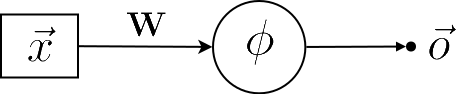
\includegraphics[width=0.4\textwidth]{pictures/figures/NN.png}
    \caption{Simplified Neural Network}
    \label{fig:NN}
\end{figure}

	For all figures under this point, $\Sigma$ node is skipped, square shape node represents input node, circle shape node represents compute node, edge with transform matrix represents weight matrix, edge without transform matrix represents identity matrix for weight matrix and arrow with small filled circle on end represents output vector. Figure \ref{fig:detail_NN}, Figure \ref{fig:withoutBiasNN}, and \ref{fig:NN} are equal.


\subsubsection{Multilayer Perceptron}\label{subsubsec:MLP}
Single layer perceptron neural network has only an input layer and an output layer such as Figure \ref{fig:NN} but multilayer perceptron (MLP) has several hidden layers between an input layer and an output layer. This part introduces to MLP by explaining neural network with one hidden layer. Let $\vec{x} \in \mathbb{R}^n$ be inputs, $\vec{h} \in \mathbb{R}^m$ be outputs from hidden layers, $\vec{c} \in \mathbb{R}^m$ be bias for hidden layers, $\vec{o} \in \mathbb{R}^l$ be outputs from an output layer, $\vec{b} \in \mathbb{R}^l$ be a bias for an output layer, $\bold{v}: \mathbb{R}^n \rightarrow \mathbb{R}^m$ be a transform matrix for hidden layers and $\bold{w}: \mathbb{R}^m \rightarrow \mathbb{R}^l$ be a transform matrix for an output layer. The activation function $\bold{f}()$ is for hidden layers and the activation function $\bold{g}()$ is for an output layer. Figure \ref{fig:MLP} shows one hidden layer MLP.

To compute output of MLP, forward-propagation is used. Forward-propagation is to pass inputs $\vec{x}$ to outputs through hidden layers \cite{murphy2012machine}. For example, the output from hidden layers on Figure \ref{fig:MLP} can be computed
$$\vec{h} = \bold{f}(\vec{x}\bold{v}+\vec{c}) = \bold{f}(\vec{X}\bold{V})$$
Then the output layer uses outputs from hidden layer as inputs. The outputs of the neural network can be computed
$$\vec{o} = \bold{g}(\vec{h}\bold{w}+\vec{b}) = \bold{g}(\vec{H}\bold{W})$$
Therefore, a final equation for two layer neural network is
$$\vec{o} = \bold{g}(\bold{h}(\vec{x}\bold{v}+\vec{c})\bold{w}+\vec{b}) = \bold{g}(\bold{h}(\vec{X}\bold{V})\bold{W})$$

\begin{figure}[t!]
    \centering
    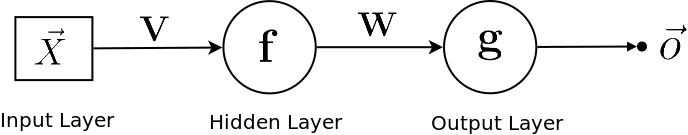
\includegraphics[width=0.5\textwidth]{pictures/figures/MLP.png}
    \caption{One Hidden Layer MLP}
    \label{fig:MLP}
\end{figure}


\subsubsection{Back-propagation}\label{subsubsec:BP}
Training neural network means finding weights and biases. Similar as forward-propagation, back-propagation is used when MLP is trained. As forward-propagation passes inputs $\vec{x}$ to outputs, back-propagation passes an error from the output layer to hidden layers \cite{murphy2012machine}. An error function $E()$ (some times called a loss function) usually uses a sum square error as follow:
$$E(\vec{y}, \vec{o}) = \frac{1}{2}\sum_{i}(y_i-o_i)^2$$
where $\vec{y}$ is an expected output from MLP.

Training neural network means finding weights and biases that make $\vec{o}$ close to $\vec{y}$. It means that training neural network needs a function of weights and biases. The train function $J()$ to train a neural network can be defined from error function $E()$. The error function $E()$ is a function of expected output and output from neural network with fixed weights and biases. Let weights and biases be changeable and the input be fixed on the error function, then the output is depends on weights and biases and the trained function $J()$ for one hidden MLP (Figure \ref{fig:MLP}) can be define below:
$$J(\bold{V}, \bold{W}) = \frac{1}{2}\sum_{i}(y_i-o_i)^2 = \frac{1}{2}\sum_{i}(y_i-g(\vec{H}\bold{W_i})^2 =\frac{1}{2}\sum_{i}(y_i-g(\bold{h}(\vec{X}\bold{V})\bold{W_i}))^2$$
where $\bold{W_i}$ is $i$th column of $\bold{W}$

The training function $J()$ for one hidden layer MLP is a function of $\bold{V}$ and $\bold{W}$ with fixed input. Again capital letter of transform matrix contains bias. So $\bold{V}$ is weights and biases for hidden layer and $\bold{W}$ is weights and biases for output layer.

To train the neural network, weights and biases are regulated. To update weights and biases, let $\vec{h'}=\vec{X}\bold{V}$ be inputs for a hidden layer activation function $\bold{f}$ and $\vec{o'}=\vec{H}\bold{W}$ be inputs for an output layer activation function $\bold{g}$. So $\vec{h}=\bold{f}(\vec{h'})=\bold{f}(\vec{X}\bold{V})$ and $\vec{o}=\bold{g}(\vec{o'})=\bold{g}(\vec{H}\bold{W})$. Let $V_{ij}$ be $i$th neuron weights in hidden layers for inputs  $X_j$ and $W_{ij}$ be $i$th neuron weight in an output layer for inputs $H_j$.

\begin{figure}[t!]
    \centering
    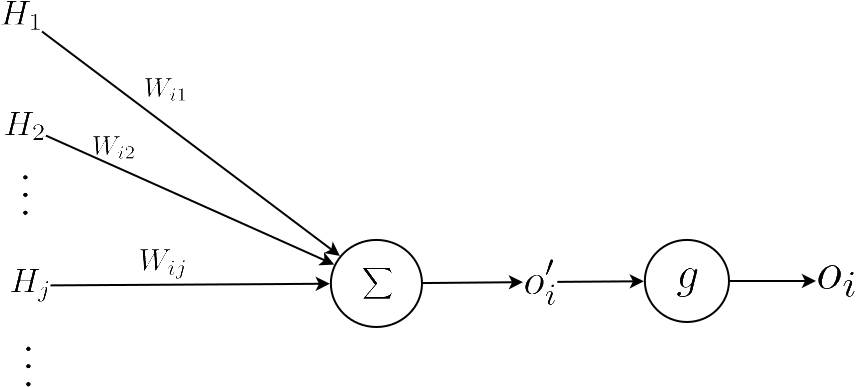
\includegraphics[width=0.7\textwidth]{pictures/figures/BP1.png}
    \caption{Back-propagation for $W_{ij}$}
    \label{fig:BP1}
\end{figure}

Let's first update $W_{ij}$ and Figure \ref{fig:BP1} shows the detail of an output layer related with ${W_{ij}}$. The updated weight ${{W_{ij}}^{next}}$ can be calculated as follow:
$${{W_{ij}}^{next}}=W_{ij} - \eta\frac{\partial J}{\partial W_{ij}}$$ where $\eta$ is a learning rate. The equation tells to remove error, updated weight should be move opposite direction of gradient of error function. The method is called 'gradient descent'.

Let's compute $\frac{\partial J}{\partial W_{ij}}$
$$
\frac{\partial J}{\partial W_{ij}}
= \frac{\partial J}{\partial o_i}\frac{\partial o_i}{\partial W_{ij}}
= \frac{\partial J}{\partial o_i}\frac{\partial o_i}{\partial o'_i}\frac{\partial o'_i}{\partial W_{ij}}
$$
So the equation has three parts.

First part is
$$
\frac{\partial o'_i}{\partial W_{ij}}
= \frac{\partial}{\partial W_{ij}}\sum_k(H_kW_{ik})
= \frac{\partial}{\partial W_{ij}}(H_jW_{ij})
= H_j
$$

Assume the activation function for an output layer is a sigmoid function $sigm()$ then the second part is
$$
\frac{\partial o_i}{\partial o'_i}
= \frac{\partial}{\partial o'_i}sigm(o'_i)
= sigm(o'_i)\{1-sigm(o'_i)\}
= o_i(1-o_i)
$$

Assume train function is sum square then the last part is
$$
\frac{\partial J}{\partial o_i}
= \frac{\partial}{\partial o_i}\frac{1}{2}\sum_k(y_k-o_k)^2
= \frac{\partial}{\partial o_i}\frac{1}{2}(y_i-o_i)^2
= -(y_i-o_i)
$$

Therefore,
$$
{{W_{ij}}^{next}}
= W_{ij} - \eta\frac{\partial J}{\partial W_{ij}}
= W_{ij} - \eta\frac{\partial J}{\partial o_i}\frac{\partial o_i}{\partial o'_i}\frac{\partial o'_i}{\partial W_{ij}}
= W_{ij} + \eta(y_i-o_i)o_i(1-o_i)H_j
$$

Before moving to update weights for hidden layer, define $\delta_i$ as follow:
$$
\delta_i
= \frac{\partial J}{\partial o'_i}
= \frac{\partial J}{\partial o_i}\frac{\partial o_i}{\partial o'_i}
$$

The $\delta_i$ is useful because it is shared when back-propagation updates all weights related with $i$th neuron. Also the $\delta_i$ is used when back-propagation updates weights on hidden layers.

\begin{figure}[t!]
    \centering
    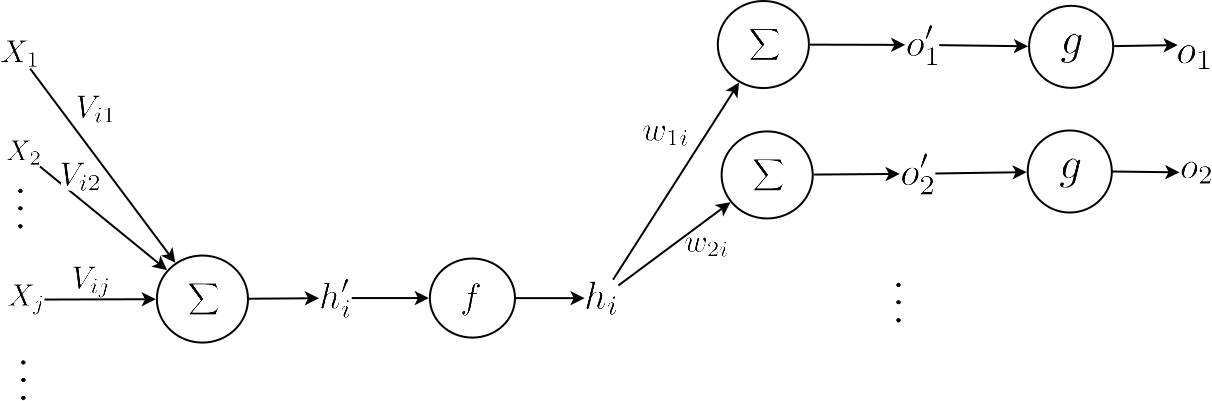
\includegraphics[width=\textwidth]{pictures/figures/BP2.png}
    \caption{Back-propagation for $V_{ij}$}
    \label{fig:BP2}
\end{figure}

The next step is to update weights in hidden layers. Let's update $V_{ij}$ and Figure \ref{fig:BP2} shows the detail of neural network related with $V_{ij}$. The updated weight ${{V_{ij}}^{next}}$ can be calculated as follow:
$${{V_{ij}}^{next}}=V_{ij} - \eta\frac{\partial J}{\partial V_{ij}}$$ where $\eta$ is a learning rate. The equation is similar as ${{W_{ij}}^{next}}$

Let's compute $\frac{\partial J}{\partial V_{ij}}$
$$
\frac{\partial J}{\partial V_{ij}}
= \frac{\partial J}{\partial h'_i}\frac{\partial h'_i}{\partial V_{ij}}
= \frac{\partial J}{\partial h_i}\frac{\partial h_i}{\partial h'_i}\frac{\partial h'_i}{\partial V_{ij}}
$$
So the equation also has three parts.

First part is
$$
\frac{\partial h'_i}{\partial V_{ij}}
= \frac{\partial}{\partial V_{ij}}\sum_k(X_kV_{ik})
= \frac{\partial}{\partial V_{ij}}(X_jV_{ij})
= X_j
$$

Assume the activation function for hidden layers is also a sigmoid function $sigm()$ then the second part is
$$
\frac{\partial h_i}{\partial h'_i}
= \frac{\partial}{\partial h'_i}sigm(h_i)
= sigm(h'_i)\{1-sigm(h'_i)\}
= h_i(1-h_i)
$$

Then the last part is
$$
\frac{\partial J}{\partial h_i}
= \sum_k(\frac{\partial J}{\partial o'_k}\frac{\partial o'_k}{\partial h_i})
= \sum_k(\delta_kw_{ki})
$$

Therefore,
$$
{{V_{ij}}^{next}}
= V_{ij} - \eta\frac{\partial J}{\partial V_{ij}}
= W_{ij} - \eta\frac{\partial J}{\partial h_i}\frac{\partial h_i}{\partial h'_i}\frac{\partial h'_i}{\partial V_{ij}}
= W_{ij} - \eta\sum_k(\delta_kw_{ki})h_i(1-h_i)X_j
$$

Notice that as forward-propagation sends outputs of a layer as inputs of the next layer, back-propagation sends error of a layer to the previous layer. For example, the $\delta_i=\frac{\partial J}{\partial o'_i}$ is error on the output layer then sends it to hidden layers. 



\subsection{Recurrent Neural Network}\label{subsec:RNN}

\subsubsection{Basic concepts of recurrent neural networks:}\label{basicRNN}
	A recurrent neural network (RNN) is a neural network that is specialized for processing a sequence of input values \cite{Goodfellow-et-al-2016}. Figure \ref{fig:RNN} illustrates abstract structure of RNN. RNN has two input. One input is from data such as normal neural network input but another input is from previous output. The property gives benefit for sequential input data. This is because past outputs affect to current output. With sequential data, previous data can affect to current data and RNN considers previous outputs for current output. It means that even input from data are equal if previous outputs are different, current output are also different.

\begin{figure}[t!]
    \centering
    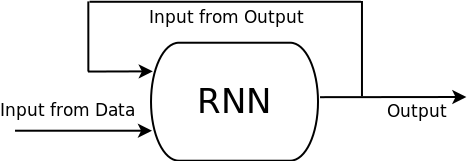
\includegraphics[width=0.5\textwidth]{pictures/figures/RNN.png}
    \caption{RNN}
    \label{fig:RNN}
\end{figure}
	
	For example, human language sentences have series of words and meaning of words is different in different context. RNN can be used for that. Another example is driving data which is used later on the paper.  Driving data are multi-dimension data with time domain. RNN can be used for the data because it is sequential data with time domain.
	
	To describe RNN in math equation, let $\vec{x^t} = \{ x_1^t, ..., x_n^t\} \in \mathbb{R}^n$ be a vector that represents the input data at time $t$, $\vec{h^t} = \{ h_1^t, ..., h_m^t\} \in \mathbb{R}^m$ be result from hidden layer on time $t$, and $\vec{o^t} = \{ o_1^t, ..., o_l^t\} \in \mathbb{R}^l$ be output on time $t$. For transform matrix, let $\bold{u}: \mathbb{R}^n \rightarrow \mathbb{R}^m$ be a transform matrix for input data, $\bold{v}: \mathbb{R}^m \rightarrow \mathbb{R}^l$ be a transform matrix for data from hidden layer, and $\bold{w}: \mathbb{R}^l \rightarrow \mathbb{R}^m$ be a transform matrix for previous output. Figure \ref{fig:unfold_RNN} illustrates unfolded RNN with defined symbols. The result from hidden layer can be calculated by 
	$$\vec{h^t} = \bold{f}(\vec{X^t}\bold{U} + \vec{O^{t-1}}\bold{W})$$ where $\bold{f}$ is activation function for hidden layer. Then the output can be calculated by
	$$\vec{o^t} = \bold{g}(\vec{H^t}\bold{V})$$ where $\bold{g}$ is activation function for output layer. Therefore, the RNN with bias is
	$$\vec{o^t} = \bold{g}(\bold{f}(\vec{x^t}\bold{u}+\vec{b_x} + \vec{o^{t-1}}\bold{w}+\vec{b_o})\bold{v}+\vec{b_h})$$ where $\vec{b_x} = \{b_{x1}, ..., b_{xm}\} \in \mathbb{R}^m$ is bias for input data, $\vec{b_o} = \{b_{o1}, ..., b_{om}\} \in \mathbb{R}^m$ is bias for previous output data, and $\vec{b_h} = \{b_{h1}, ..., b_{hl}\} \in \mathbb{R}^l$ is bias for data from hidden layer. 
	
\begin{figure}[t!]
    \centering
    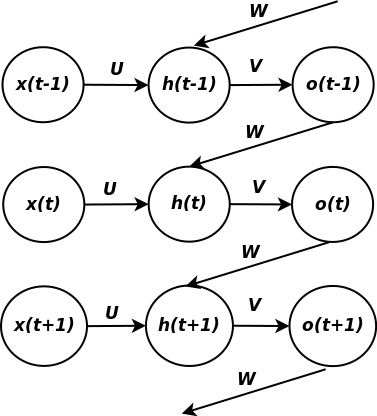
\includegraphics[width=0.65\textwidth]{pictures/figures/unfold_RNN.png}
    \caption{Unfold RNN}
    \label{fig:unfold_RNN}
\end{figure}

	RNN is not always like Figure \ref{fig:unfold_RNN}. Input from previous output can be replaced by result of previous hidden layer. The main idea of RNN is when neural network decides current output it considers previous state.
	
	
\subsubsection{Long Short Term Memory (LSTM) networks:}\label{LSTM}
	Basic RNN has the problems of long term dependency. When RNN passes previous output for current output, some information in the input might not need or might need for future. RNN does not have ability to filter unnecessary information or to store necessary information. Long Short Term Memory (LSTM) neural network can handle these problems.
	
	LSTM is a type of RNN and introduced by Hochreiter and Schmidhuber \cite{hochreiter1997long}. LSTM solves long term dependency problems in RNN by memory cells. LSTM manages memory cells as storage of knowledge. LSTM filters unnecessary information from memory cells and records necessary information on memory cells.
	
	The structure of LSTM consists of four gates: forget gate, input gate, input modulation gate, and output gate. Each gates have different purpose and Christopher Olah's blog \footnote{\url{http://colah.github.io/posts/2015-08-Understanding-LSTMs}} develops an intuition for concept of LSTM and explains purpose of each gates. The paper \cite{zaremba2014recurrent}  describes LSTM in mathematical term. Let us first provide an intuitive description of how LSTM work by following Christopher Olah's blog, before providing a more in-depth formalization.
		
%	Bengio mentioned on his paper \cite{bengio2009learning} that each layers in deep neural network should have {\color{red} a} purpose. LSTM can be divided to four layers: forget gate, input gate, input modulation gate, and output gate. Each layers have different purpose {\color{red} [santi: this paragraph does not flow very well], even if Bengio mentioned it, why is it important? you need to explain WHY is it that each layer should have a purpose. Otherwise, we just have to blindly believe in Bengio :)}.

	
\begin{enumerate}
\item An intuitive explanation of LSTMs:
	
	The easiest way to understand LSTM is to understand memory cell and purpose of four different gates. Memory cell makes LSTM different from RNN. Memory cell stores important information and filters unimportant information for future. Three of four gates are involved in the memory cells to store and filter information.
		
	The first gate affecting to memory cells is forget gate. The forget gate decides unnecessary data from input data and previous output then applies it to memory cells. Other two gates are input gate and input modulation gate and these also affect to memory cells. The two gates decide what information remember then apply it to memory cells. The last gate is output gate and it does not directly affect to memory cells. Output gate also has two inputs from input data and previous output, and output from output gate is multiplied by memory cells to make final output. Figure \ref{fig:LSTM} illustrates LSTM neural network with four gates and next part describes more detail of LSTM and the figure in mathematical terms.

\begin{figure}[t!]
    \centering
    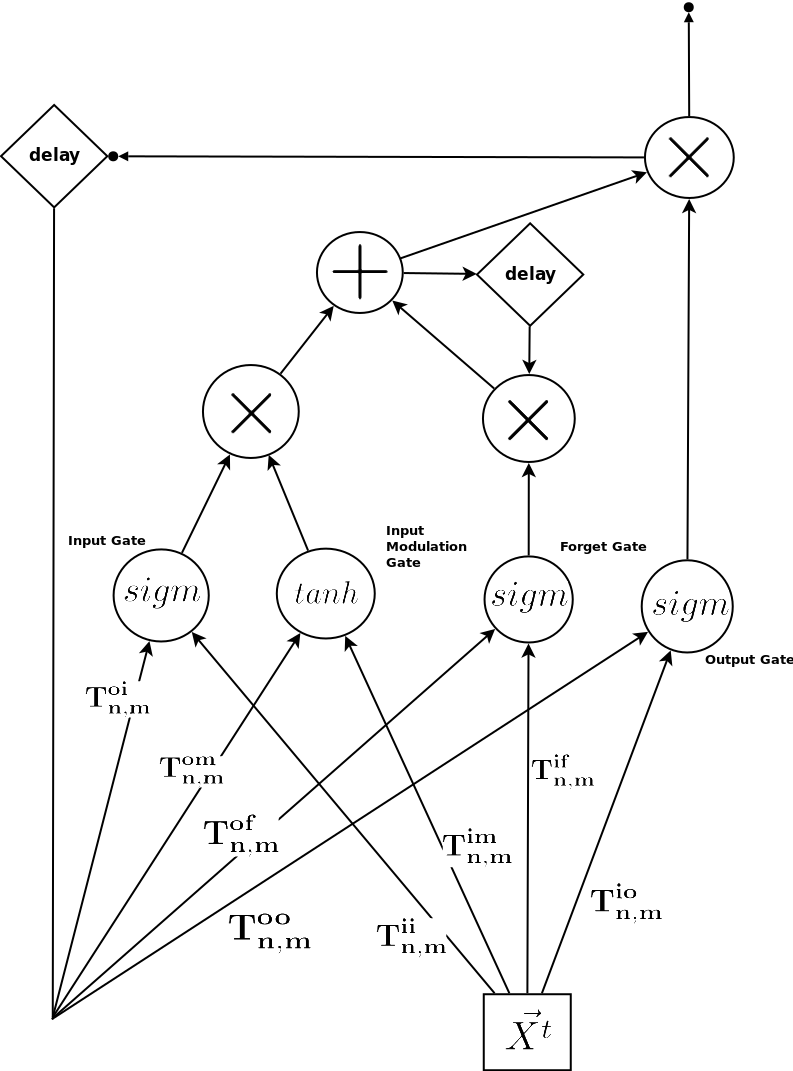
\includegraphics[width=0.75\textwidth]{pictures/figures/LSTM.png}
    \caption{LSTM}
    \label{fig:LSTM}
\end{figure}
		
		% It consists of sigmod {\color{red} [santi: instead of saying ``It consists of sigmod'', you should say something like ``The units in this layer use a sigmoid activation function'' (same comment for all the other layers below)]} layer with previous output and current input data {\color{red} [santi: a reader not familiar with LSTMs will not know what is ``previous output'' or ``current input'', so you need a figure that explains it]}. The result of the forget gate is multiplied by previous cell state to build current cell state.
		
		% The second layer is input gate and also consists of sigmod layer with previous output and current input data. The result of the input gate is multiplied by the result of input modulation gate then it affects to cell state {\color{red} [santi: all of these terms should appear in a figure, otherwise, a reader not familiar with it will not understand what you are saying. But also, even if you have a figure, you need to explain what each term is, e.g., explain what is ``input modulation'', what is ``cell state'', etc.]}. The meaning of input gate is to decide{\color{red} \st{s}} what data to remember.
		
		% The third layer is input modulation gate. It consists of tanh with previous output and current input. It is multiplied by the result of second layer and affects to current cell state.
		
		% The last layer is output gate. The layer decides what data should be passed to current output from previous output and current input. the output gate also consists of sigmoid with two inputs: last output and current input. The result of the layer is multiplied by current cell state passed tanh.
	
\item Modeling LSTMs in mathematical terms:
	
	To describe LSTM in mathematical terms, let $\vec{x^t} = \{ x_1^t, ..., x_n^t\} \in \mathbb{R}^n$ be a vector that represents the input data at time $t$, $\vec{i^t} = \{i_1^t, ..., i_m^t\} \in \mathbb{R}^m$ be result from input gate on time $t$, $\vec{m^t} = \{m_1^t, ..., m_m^t\} \in \mathbb{R}^m$ be result from input modulation gate on time $t$, $\vec{f^t} = \{f_1^t, ..., f_m^t\} \in \mathbb{R}^m$ be result from forget gate on time $t$, $\vec{o^t} = \{o_1^t, ..., o_m^t\} \in \mathbb{R}^m$ be result from output gate on time $t$, $\vec{c^t} = \{c_1^t, ..., c_m^t\} \in \mathbb{R}^m$ be memory cells on time $t$, and $\vec{h^t} = \{h_1^t, ..., h_m^t\} \in \mathbb{R}^m$ be final result on time $t$.
Each gates have transform matrices for inputs. Let $\bold{t_{n,m}}: \mathbb{R}^n \rightarrow \mathbb{R}^m$ be a transform matrix from $n$ dimension to $m$ dimension. Let $\bold{t_{n,m}^{ii}}$ be a transform matrix for input from data in input gate, $\bold{t_{m,m}^{oi}}$ be a transform matrix for input from previous output in input gate, $\bold{t_{n,m}^{im}}$ be a transform matrix for input from data in input modulation gate, $\bold{t_{m,m}^{om}}$ be a transform matrix for input from previous output in input modulation gate, $\bold{t_{n,m}^{if}}$ be a transform matrix for input from data in forget gate, $\bold{t_{m,m}^{of}}$ be a transform matrix for input from previous output in forget gate, $\bold{t_{n,m}^{io}}$ be a transform matrix for input from data in output gate, $\bold{t_{m,m}^{oo}}$ be a transform matrix for input from previous output in output gate.

	The result of each gates are computed as following:
	$$\vec{i^t} = \bold{sigm}(\vec{X^t}\bold{T_{n,m}^{ii}} + \vec{H^{t-1}}\bold{T_{m,m}^{oi}})$$
	Input gate uses sigmoid function $\bold{sigm()}$ for activation function
	$$\vec{m^t} = \bold{tanh}(\vec{X^t}\bold{T_{n,m}^{im}} + \vec{H^{t-1}}\bold{T_{m,m}^{om}})$$
	Input modulation gate uses tanh function $\bold{tanh()}$ for activation function.
	$$\vec{f^t} = \bold{sigm}(\vec{X^t}\bold{T_{n,m}^{if}} + \vec{H^{t-1}}\bold{T_{m,m}^{of}})$$
	Forget gate uses sigmoid function $\bold{sigm()}$ for activation function.
	$$\vec{o^t} = \bold{sigm}(\vec{X^t}\bold{T_{n,m}^{io}} + \vec{H^{t-1}}\bold{T_{m,m}^{oo}})$$
	Output gate uses sigmoid function $\bold{sigm()}$ for activation function.

	Memory cells are computed as
	$$\vec{c^t} = \vec{i^t} * \vec{m^t} + \vec{f^t} * \vec{c^{t-1}}$$
		
	And final result is computed as
	$$\vec{h^t} = \vec{c^t} * \vec{o^t}$$
		
	Where $*$ is component-wise multiplication of two vectors.
\end{enumerate}
	
	LSTM neural network described above is one example of LSTMs. There are many other LSTMs but all LSTMs has memory cells to store information for long term memory and has four gates: input, input modulation, forget, and output gate.



\subsection{Auto-encoder}\label{subsec:AE}

This subsection introduces Auto-encoder and different kind of Auto-encoder: undercomplete Auto-encoder, overcomplete Auto-encoder, and multilayer Auto-encoder.

% and summarizes 'Reducing the dimensionality of data with neural networks' by Hinton \cite{hinton2006reducing}. The paper introduces to the method to reduce high dimensional data by neural networks named auto-encoder. The result of the paper shows that reducing dimension by auto-encoder gives better performance than PCA.

\subsubsection{Basic Auto-encoder}\label{subsubsec:BAE}
An Auto-encoder (AE) is defined as a neural network that is trained to attempt to copy its input to its output \cite{Goodfellow-et-al-2016}. It means that AE takes input and sends it as output. However, AE does not directly send input to output. AE has two layers: encode layer and decode layer. Figure \ref{fig:AE} illustrates abstract structure of AE. Purpose of AE is to make output from decode same as input.

\begin{figure}[t!]
    \centering
    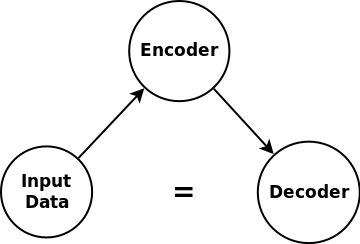
\includegraphics[width=0.5\textwidth]{pictures/figures/AE.png}
    \caption{Abstract structure of Auto-encoder}
    \label{fig:AE}
\end{figure}

To describe AE, let $\vec{x} = \{x_1, ..., x_n\} \in \mathbb{R}^n$ be input, $\vec{e} = \{e_1, ..., e_m\} \in \mathbb{R}^m$ be output from encoder layer, and $\vec{d} = \{d_1, ..., d_n\} \in \mathbb{R}^n$ be output from decoder layer. For transform matrix, let $\bold{u}: \mathbb{R}^n \rightarrow \mathbb{R}^m$ be a transform matrix for encode layer, $\bold{v}: \mathbb{R}^m \rightarrow \mathbb{R}^n$ be a transform matrix for decode layer. Usually AE uses sigmoid for activation function. Figure \ref{fig:basic_AE} describes AE.

\begin{figure}[t!]
    \centering
    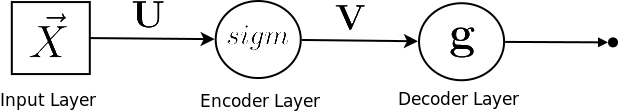
\includegraphics[width=0.5\textwidth]{pictures/figures/basic_AE.png}
    \caption{Basic Auto-encoder}
    \label{fig:basic_AE}
\end{figure}

The output of encoder is
$$\vec{e} = \bold{f}(\vec{X}\bold{U})$$
where $\bold{f}$ is the activation function for encoder layer. It is usually sigmoid function.

The output of decoder is
$$\vec{d} = \bold{g}(\vec{E}\bold{V})$$
where $\bold{g}$ is the activation function for decoder layer. It is usually sigmoid or linear function.

The purpose of AE copies input as output. Therefore, the error function is calculated by
$$E(\vec{x}, \vec{d}) = E(\vec{x}, \bold{g}(\vec{E}\bold{V})) = E(\vec{x}, \bold{g}(\bold{f}(\vec{x}\bold{u}+\vec{b_e})\bold{v}+\vec{b_d}))$$
Where $\vec{b_e} = \{b_{e1}, ..., b_{em}\} \in \mathbb{R}^m$ is bias for encoder layer and $\vec{b_d} = \{b_{d1}, ..., b_{dm}\} \in \mathbb{R}^n$ is bias for decoder layer.

AE seems not useful because it only tries to copy input. However, AE is usually used with other neural network and other neural network uses data from encoder layer of AE not from decoder layer. Making similar values of input and decoder output guarantees that result from encode layer contains all information of input. It means that AE can represent same information of input data in different dimension. When dimension of encoder is higher than dimension of input, it is called overcomplete Auto-encoder. When dimension of encoder is lower than dimension of input, it is called undercomplete Auto-encoder.

On this paper and experiment, undercomplete AE is used for reducing input dimension. Undercomplete AE is often compared with principal components analysis (PCA) because both methods reduce dimension. The paper \cite{hinton2006reducing} compares undercomplete AE and PCA. The result on the paper is that undercomplete AE could keep more information than PCA. It means that reducing data to low dimension by undercomplete AE gives better performance. However, training AE takes long time than computing information gain for PCA.

% When auto-encoder is traind, it has two layers: encode and decode. The encode layer receives input and passes output in lower dimension data to decode layer. The decode layer recovers dimension to input data dimention from output of encode layer. The error of auto-encoder is measured by difference between input data and output from decode layer. In other words, encoder layer compresses input data and decoder layer decompresses data from encoder layer that should be similar as original input data. That methods guarantees that the data from encoder layer keeps almost all properties of input data in lower dimension. That is the reason why output data from decode layer is similar as original input data. In math, relationship between encoder and decoder layer is similar as inverse matrix of each other.


\subsubsection{Multilayer Auto-encoder}\label{subsubsec:MAE}
	Sometimes AE is designed with multiple encoder and decoder layers to reduce dimension. Figure \ref{fig:MAE} shows multilayer auto-encoder (MAE). However, it is difficult to find the all weights of encoder and decoder in MAE because all weights are initialized with random numbers and it makes difficult to find optimize weights \cite{zaremba2014recurrent}. So if the initial weights are close to optimize weights, training algorithm gradient descent can find optimize weights. The paper \cite{zaremba2014recurrent} shows "pretraining" method to initialize good weights. 
	
\begin{figure}[t!]
    \centering
    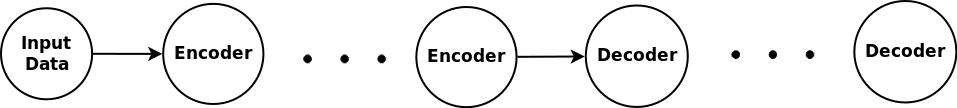
\includegraphics[width=0.75\textwidth]{pictures/figures/MAE.png}
    \caption{Multilayer Auto-encoder}
    \label{fig:MAE}
\end{figure}

\begin{figure}[t!]
    \centering
    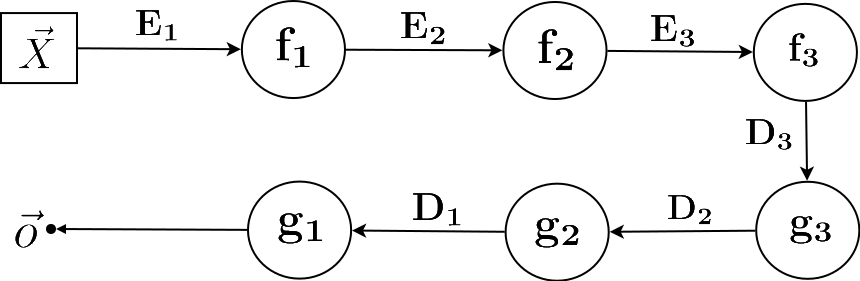
\includegraphics[width=0.75\textwidth]{pictures/figures/example_MAE.png}
    \caption{Multilayer Auto-encoder Example}
    \label{fig:example_MAE}
\end{figure}

	Pretraining is to train each layer separately before train whole layers. For example, Figure \ref{fig:example_MAE} has three encoder and decoder layers. Let $\vec{x} \in \mathbb{R}^n$ be input vector, $\bold{e_1}: \mathbb{R}^n \rightarrow \mathbb{R}^m$ be transform matrix for first encoder layer, $\bold{e_2}: \mathbb{R}^m \rightarrow \mathbb{R}^l$ be transform matrix for second encoder layer, $\bold{e_3}: \mathbb{R}^l \rightarrow \mathbb{R}^k$ be transform matrix for third encoder layer, $\bold{d_1}: \mathbb{R}^m \rightarrow \mathbb{R}^n$ be transform matrix for first decoder layer, $\bold{d_2}: \mathbb{R}^l \rightarrow \mathbb{R}^m$ be transform matrix for second decoder layer, $\bold{d_3}: \mathbb{R}^k \rightarrow \mathbb{R}^l$ be transform matrix for third decoder layer, and $\vec{o} \in \mathbb{R}^n$ be output vector.

\begin{figure}[t!]
    \centering
    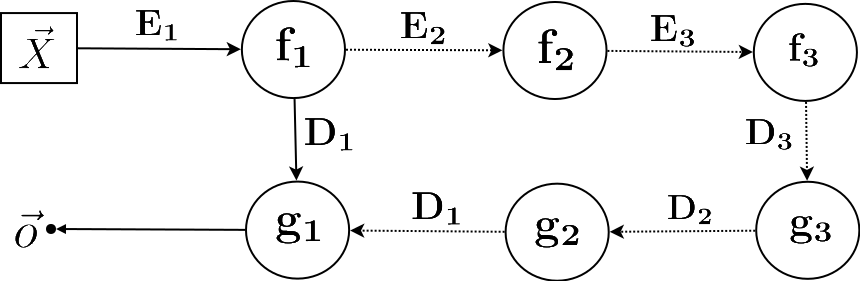
\includegraphics[width=0.75\textwidth]{pictures/figures/train_MAE1.png}
    \caption{Pretraining First Step}
    \label{fig:train_MAE1}
\end{figure}

\begin{figure}[t!]
    \centering
    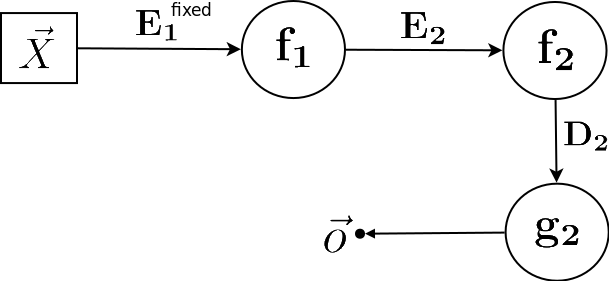
\includegraphics[width=0.75\textwidth]{pictures/figures/train_MAE2.png}
    \caption{Pretraining Second Step}
    \label{fig:train_MAE2}
\end{figure}

\begin{figure}[t!]
    \centering
    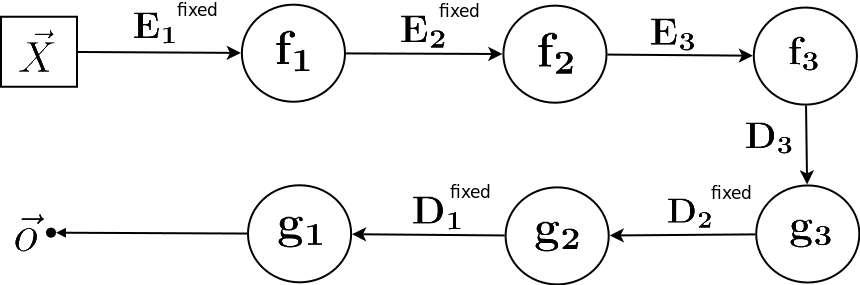
\includegraphics[width=0.75\textwidth]{pictures/figures/train_MAE3.png}
    \caption{Pretraining Thrid Step}
    \label{fig:train_MAE3}
\end{figure}

	In this case, pretraining has three steps because it has three encoder and decoder layers. Figure \ref{fig:train_MAE1} shows train of first encoder and decoder layer. While first encoder and decoder layer are trained, rest encoder and decoder are ignored. So error function is
$$E(\vec{x}, \bold{g_1}(\bold{f_1}(\vec{X}\bold{E_1})\bold{D_1}))$$
Figure \ref{fig:train_MAE2} shows train of second encoder and decoder layer. While second encoder and decoder layer are trained, transform matrix $\bold{e_1}$ and $\bold{d_1}$ are fixed because two transform matrix are already trained previous step. So error function is
$$E(\vec{x}, \bold{g_1}(\bold{g_2}(\bold{f_2}(\bold{f_1}(\vec{X}\bold{E_1^{fixed}})\bold{E_2})\bold{D_2})\bold{D_1^{fixed}}))$$
The last step is Figure \ref{fig:train_MAE3} and it trains third encoder and decoder. During this, first and second encoder and decoder weights are fixed. So error function is
$$E(\vec{x}, \bold{g_1}(\bold{g_2}(\bold{g_3}(\bold{f_3}(\bold{f_2}(\bold{f_1}(\vec{X}\bold{E_1^{fixed}})\bold{E_2^{fixed}})\bold{E_3})\bold{D_3})\bold{D_2^{fixed}})\bold{D_1^{fixed}}))$$
	
	After finishing pretraining step, all weights are close enough to optimal weights for train algorithm to find optimize answer when it train whole neural network. So error function training whole network is
$$E(\vec{x}, \bold{g_1}(\bold{g_2}(\bold{g_3}(\bold{f_3}(\bold{f_2}(\bold{f_1}(\vec{X}\bold{E_1})\bold{E_2})\bold{E_3})\bold{D_3})\bold{D_2})\bold{D_1}))$$


\section{Deep Learning Libraries}\label{sec:DLL}
This section introduces to three popular libraries for deep learning.

\subsection{Tensorflow}
Tensorflow \footnote{\url{https://www.tensorflow.org/}} is an open source software library for numerical computation using data flow graphs. The biggest difference from other libraries is that Tensorflow treats all operator as a node. For example, multiplication, addition, or sigmoid function are treated as a node.  This helps developers intuitively build neural network. Another strong points is TensorBoard. TensorBoard is a tool for Tensorflow to visualize neural networks built in Tensorflow. Also developers can review how neural networks are trained from TensorBoard because TensorBoard visualizes logs to track all parameters while neural networks are trained.

The most famous example of Tensorflow is AlphaGo \footnote{\url{https://cloudplatform.googleblog.com/2016/05/Google-supercharges-machine-learning-tasks-with-custom-chip.html}}. Google engineer teams build AlphaGo with Tensorflow and the AlphaGo runs on Tensor Processing Unit (TPU).


\subsection{Theano}
Theano \footnote{\url{http://deeplearning.net/software/theano/}} is a Python library for machine learning. It integrates with Numpy and dynamically generates C code. Theano has many defined computations (called Op) and Theano allows to extend custom Ops written in C code.

Theano has more example codes and more stable than Tensorflow. This is because Tensorflow is newer than Theano and APIs of Tensorlfow keep changing. For example, many APIs in Tensorflow 1.x have different interfaces from APIs in Tensorflow 0.x.


\subsection{DL4J}
DL4J \footnote{\url{https://deeplearning4j.org/}} is open source, distributed deep-learning library for Java and Scala under the Apache 2.0 license. To compare with other deep learning libraries, DL4J can easily interact with Hadoop and Spark so neural networks built in DL4J can be used for big data.


\section{Machine Learning with Driving Data}\label{sec:MLDD}

% ####################################################################################################################################
\chapter{Data Set}
% ####################################################################################################################################

Data was collected in the high-fidelity simulator \cite{lee2017learning} of the Center for Injury Research Prevention Studies at the \textit{Children's Hospital of Philadelphia} (CHOP). The driving simulator provides an environment similar to real driving to test users. It has a 160 degree front view, rear-view, left side, and right side mirror images. It also features a full car chassis with active pedals, steering wheel, and a full dashboard with even audio equipment.

The experiments on this paper use 16 traces from 4 drivers: 2 people are expert drivers and 2 people are inexpert drivers. Each person drove four different tracks and each track represent different traffic situations and interactions with other vehicles. Each track has multiple instances of three scenarios that have been found to result in a high likelihood of crashing for 16-18 year- old teen drivers driving alone or with a peer passenger according to the NMVCCS (National Motor Vehicle Crash Causation Survey): 1) turning into opposite directions (turning left), 2) right roadside departure, and 3) rear-end events \cite{mcdonald2012using}. Thus, this results on a dataset that contains 8 traces of expert drivers, and 8 traces of inexpert drivers.

The simulator records 100 features which include car status: velocity, steer, Brake, throttle and etc. and include environment status features such as the current speed limit, whether the driver is instructed to make the next left or right turn, etc. These data is collected at 60Hz. The traces vary in length from 26298 to 51295, with an average of 33224.6875 instances. The specific lengths of each trace are shown on Table \ref{tbl:traces}

In this paper, we used two versions of the collected data set. A first version ({\em raw dataset}) contains 98 of the 100 features collected by the driving simulator (the two features that are removed are time stamps). A second version ({\em filtered dataset}) contains only 23 features. These 23 features were manually selected as are those that are most important for the classification task at hand. Reducing size of features helps save time to train neural network.

\begin{table}[!t]
\centering
\caption{Length of each of the traces used in our experiments.}
\label{tbl:traces}
\begin{tabular}{|l|l|l|l|}
\hline
{\em Trace}   & {\em Driver}    & {\em Track}  & {\em Length} \\ \hline
Trace0  & Expert0   & Track0 & 50029  \\
Trace1  & Expert0   & Track1 & 26375  \\
Trace2  & Expert0   & Track2 & 29629  \\
Trace3  & Expert0   & Track3 & 26298  \\
Trace4  & Expert1   & Track0 & 51295  \\
Trace5  & Expert1   & Track1 & 26674  \\
Trace6  & Expert1   & Track2 & 29680  \\
Trace7  & Expert1   & Track3 & 27075  \\
Trace8  & Inexpert0 & Track0 & 49691  \\
Trace9  & Inexpert0 & Track1 & 30058  \\
Trace10 & Inexpert0 & Track2 & 26441  \\
Trace11 & Inexpert0 & Track3 & 27373  \\
Trace12 & Inexpert1 & Track0 & 47658  \\
Trace13 & Inexpert1 & Track1 & 29380  \\
Trace14 & Inexpert1 & Track2 & 26684  \\
Trace15 & Inexpert1 & Track3 & 27255  \\ \hline
\end{tabular}
\end{table}


% ####################################################################################################################################
\chapter{Technical Approach}
% ####################################################################################################################################

This chapter covers technical methods for experiments on the paper also introduces to three different neural network used for the experiments.


\section{Cross Validation}
Cross validation (CV) is used to validate model when data is not enough \cite{Goodfellow-et-al-2016}. CV divides data set to $K$ folds then applies $i$th fold as test set and other folds as train set to target model. Experiments on the paper use 16 traces but it is not enough to train neural network. CV can be used to validate neural network model and compare performance of three different models. The 16 traces dataset is divided to 4 folds. Each folds contain two traces from expert and two traces from inexpert. The neural networks are trained four times with different train (3 folds) and test (1 fold) set. Figure \ref{fig:CV} shows four folds cross validation. Red color is the fold for testing and other folds are for training. 

\begin{figure}[t!]
    \centering
    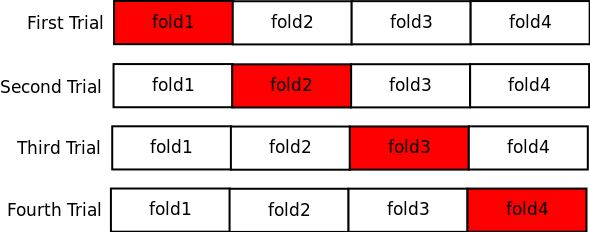
\includegraphics[width=0.7\textwidth]{pictures/figures/CV.png}
    \caption{Cross Validation}
    \label{fig:CV}
\end{figure}


\section{LSTM}
The LSTM neural network is used on three different neural network models to classify expert or inexpert driver because the data has time domain and LSTM gives good performance for serial data. On the paper, LSTM neural network is built with 16, 32, 64, 128, and 256 number of hidden neurons. The output from LSTM is sent to output layer which has two neurons. By using softmax, output from two neurons is classified. If it has [0, 1], it is classified to expert. Otherwise, it is classified to inexpert.

Figure \ref{fig:exp_NN1} shows first neural network model ({\em first model}) on the paper. Its input is {\em filtered dataset} which has 23 chosen features. The {\em filtered dataset} is feed directly to LSTM then the result is passed to output layer.

\begin{figure}[t!]
    \centering
    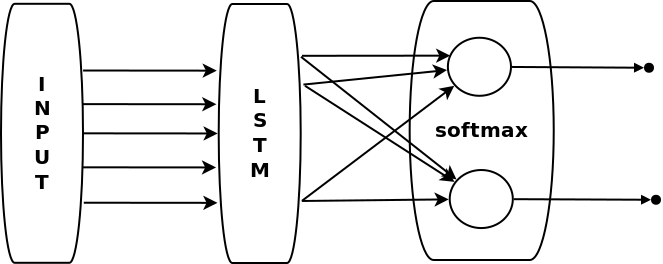
\includegraphics[width=0.7\textwidth]{pictures/figures/exp_NN1.png}
    \caption{First experiment NN}
    \label{fig:exp_NN1}
\end{figure}


\section{Auto-encoder}
The {\em raw dataset} has 98 features and it takes too much time to train nerual network if all 98 features are used. AE can solve the problem by reducing dimensions. 

\subsection{Single layer Auto-encoder}
Figure \ref{fig:exp_NN2} shows second neural network model ({\em second model}) on the paper. The {\em second model} is added by one AE layer from {\em first model}. The purpose of the AE layer is to reduce 98 features to 25 features on {\em raw dataset}. Notice that the figure only has encoder because after training AE, only encoder is used to reduce dimensions. The output from encoder is passed to LSTM.

\begin{figure}[t!]
    \centering
    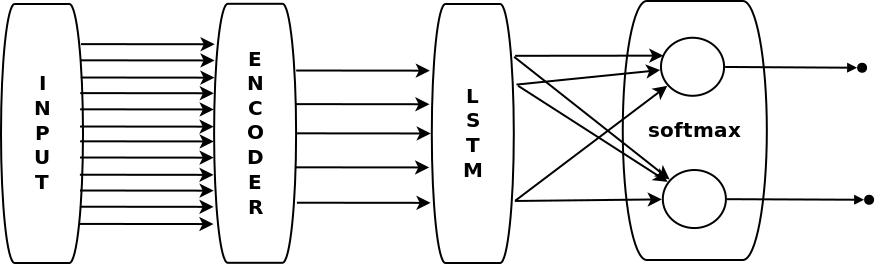
\includegraphics[width=0.8\textwidth]{pictures/figures/exp_NN2.png}
    \caption{Second experiment NN}
    \label{fig:exp_NN2}
\end{figure}


\subsection{Multiple layer Auto-encoder}
Figure \ref{fig:exp_NN3} shows third neural network model ({\em third model}) on the paper. To compare performance between single layer AE and multiple layer AE, the {\em third model} has three layers of AE.  First AE reduces 98 dimensions to 75 dimensions, second AE reduces 75 dimensions to 50 dimensions and the last AE reduces 50 dimensions to 25 dimensions. The figure describes it with three encoder layers.

\begin{figure}[t!]
    \centering
    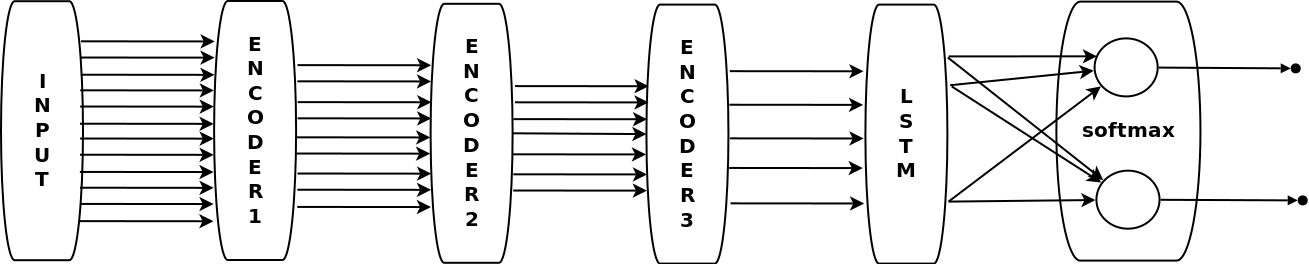
\includegraphics[width=\textwidth]{pictures/figures/exp_NN3.png}
    \caption{Third experiment NN}
    \label{fig:exp_NN3}
\end{figure}


\section{Sampling and Standardization}
The simulator records 60 samples per second. It is too often recorded. The dataset is re-sampled by three different periods: 1 over 10, 1 over 20, and 1 over 50. When it is re-sampled, three methods are used. First method chooses last sample of period, second method computes mean of data in period, and third method applies Gaussian filter. For third method, window size is 11, 21, and 51 for each period.



% ####################################################################################################################################
\chapter{Experiment Result}
% ####################################################################################################################################


\begin{figure}[H]
    \centering
    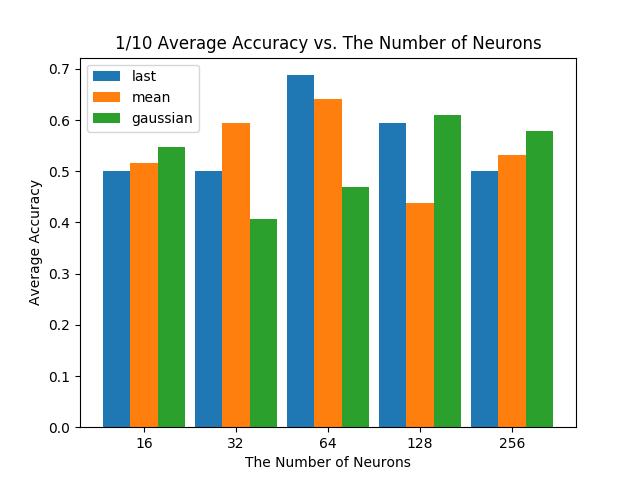
\includegraphics[width=0.75\textwidth]{pictures/result_pictures/filtered_1_10_result.png}
    \caption{Accuracy}
    \label{fig:Accuracy}
\end{figure}


\begin{table}[H]
\centering
\begin{tabular}{|l|l|l|l|l|l|l|}
\hline
                       &      & \multicolumn{5}{l|}{The number of neurans} \\ \hline
Test                   & n    & 16    & 32    & 64      & 128      & 256   \\ \hline
\multirow{4}{*}{1}     & 1    & 0.5   & 0.25  & 1.0     & 0.5      & 0.5   \\ \cline{2-7} 
                       & 2    & 0.75  & 0.75  & 0.5     & 0.5      & 0.5   \\ \cline{2-7} 
                       & 3    & 1.0   & 0.5   & 0.5     & 0.75     & 0.5   \\ \cline{2-7} 
                       & 4    & 0.5   & 0.5   & 0.75    & 0.5      & 0.5   \\ \hline
\multirow{4}{*}{2}     & 1    & 0.5   & 0.75  & 0.75    & 0.75     & 0.75  \\ \cline{2-7} 
                       & 2    & 0.25  & 0.25  & 0.75    & 0.5      & 0.25  \\ \cline{2-7} 
                       & 3    & 0.5   & 0.5   & 0.25    & 0.75     & 0.25  \\ \cline{2-7} 
                       & 4    & 0.25  & 0.25  & 0.5     & 0.25     & 0.75  \\ \hline
\multirow{4}{*}{3}     & 1    & 0.75  & 0.25  & 1.0     & 0.75     & 0.25  \\ \cline{2-7} 
                       & 2    & 0.25  & 0.5   & 0.75    & 0.5      & 1.0   \\ \cline{2-7} 
                       & 3    & 0.5   & 0.75  & 0.75    & 0.5      & 0.5   \\ \cline{2-7} 
                       & 4    & 0.5   & 0.25  & 0.75    & 0.75     & 0.5   \\ \hline
\multirow{4}{*}{4}     & 1    & 0.75  & 0.5   & 0.5     & 0.5      & 0.5   \\ \cline{2-7} 
                       & 2    & 0.25  & 0.5   & 0.5     & 1.0      & 0.25  \\ \cline{2-7} 
                       & 3    & 0.0   & 0.75  & 1.0     & 0.75     & 0.25  \\ \cline{2-7} 
                       & 4    & 0.75  & 0.75  & 0.75    & 0.25     & 0.75  \\ \hline
\multicolumn{2}{|l|}{Average} & 0.5   & 0.5   & 0.6875  & 0.59375  & 0.5   \\ \hline
\end{tabular}
\caption{Raw 1/10 Result Summary}
\label{Raw 1/10 Result Summary}
\end{table}


% ####################################################################################################################################
\chapter{Conclusion and Future work}
% ####################################################################################################################################
Conclusion and Future work\\



\end{thesis}

\bibliography{references.bib}

\end{document}
\endinput

